\documentclass[8pt,aspectratio=169]{beamer}
\usetheme{Madrid}
\usepackage{graphicx}
\usepackage{booktabs}
\usepackage{adjustbox}
\usepackage{multicol}
\usepackage{amsmath}
\usepackage{listings}
\usepackage{xcolor}

% Color definitions
\definecolor{mlblue}{RGB}{0,102,204}
\definecolor{mlpurple}{RGB}{51,51,178}
\definecolor{mllavender}{RGB}{173,173,224}
\definecolor{mllavender2}{RGB}{193,193,232}
\definecolor{mllavender3}{RGB}{204,204,235}
\definecolor{mllavender4}{RGB}{214,214,239}
\definecolor{mlorange}{RGB}{255, 127, 14}
\definecolor{mlgreen}{RGB}{44, 160, 44}
\definecolor{mlred}{RGB}{214, 39, 40}
\definecolor{mlgray}{RGB}{127, 127, 127}

% Additional colors for template compatibility
\definecolor{lightgray}{RGB}{240, 240, 240}
\definecolor{midgray}{RGB}{180, 180, 180}

% Apply custom colors to Madrid theme
\setbeamercolor{palette primary}{bg=mllavender3,fg=mlpurple}
\setbeamercolor{palette secondary}{bg=mllavender2,fg=mlpurple}
\setbeamercolor{palette tertiary}{bg=mllavender,fg=white}
\setbeamercolor{palette quaternary}{bg=mlpurple,fg=white}

\setbeamercolor{structure}{fg=mlpurple}
\setbeamercolor{section in toc}{fg=mlpurple}
\setbeamercolor{subsection in toc}{fg=mlblue}
\setbeamercolor{title}{fg=mlpurple}
\setbeamercolor{frametitle}{fg=mlpurple,bg=mllavender3}
\setbeamercolor{block title}{bg=mllavender2,fg=mlpurple}
\setbeamercolor{block body}{bg=mllavender4,fg=black}

% Remove navigation symbols
\setbeamertemplate{navigation symbols}{}

% Clean itemize/enumerate
\setbeamertemplate{itemize items}[circle]
\setbeamertemplate{enumerate items}[default]

% Reduce margins for more content space
\setbeamersize{text margin left=5mm,text margin right=5mm}

% Command for bottom annotation (Madrid-style)
\newcommand{\bottomnote}[1]{%
\vfill
\vspace{-2mm}
\textcolor{mllavender2}{\rule{\textwidth}{0.4pt}}
\vspace{1mm}
\footnotesize
\textbf{#1}
}

% TikZ and pgfplots packages
\usepackage{tikz}
\usepackage{pgfplots}
\pgfplotsset{compat=1.18}
\usetikzlibrary{arrows.meta, positioning, shapes.geometric, shapes.symbols, calc, decorations.pathmorphing}

\title{Blockchain Fundamentals: A Visual Introduction}
\subtitle{Standalone Mini-Lecture}
\author{Prof.~Dr.~Joerg Osterrieder}
\institute{University Lecture Series}
\date{\today}

\begin{document}

% ==================== FRAME 1: TITLE ====================
\begin{frame}[plain]
\vspace{2cm}
\begin{center}
{\Huge\color{mlpurple} Blockchain Fundamentals}\\[0.4cm]
{\Large\color{mlblue} A Visual Introduction}\\[0.3cm]
{\normalsize Standalone Mini-Lecture}\\[0.3cm]
\textcolor{mlgray}{\rule{6cm}{0.4pt}}\\[0.3cm]
{\small\itshape ``A digital chain of trust''}\\[1.5cm]
{\normalsize Prof.~Dr.~Joerg Osterrieder}\\[0.2cm]
{\small University Lecture Series}\\[0.2cm]
{\small \today}
\end{center}
\end{frame}

% ==================== FRAME 2: THE TRUST PROBLEM (Comic Strip 1) ====================
\begin{frame}{The Trust Problem}
\begin{center}
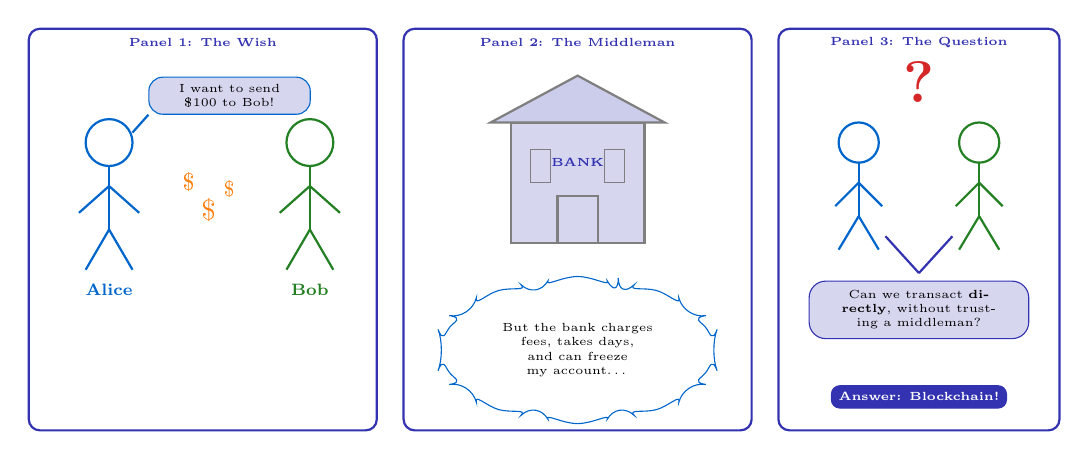
\begin{tikzpicture}[scale=0.85, every node/.style={transform shape}]

% --- Panel 1: Alice and Bob ---
\draw[mlpurple, thick, rounded corners=4pt] (-7.2,-2.8) rectangle (-2.0,3.2);
\node[font=\tiny\bfseries, mlpurple] at (-4.6,3.0) {Panel 1: The Wish};

% Alice stick figure
\draw[mlblue, thick] (-6.0,1.5) circle (0.35); % head
\draw[mlblue, thick] (-6.0,1.15) -- (-6.0,0.2); % body
\draw[mlblue, thick] (-6.0,0.85) -- (-6.45,0.45); % left arm
\draw[mlblue, thick] (-6.0,0.85) -- (-5.55,0.45); % right arm
\draw[mlblue, thick] (-6.0,0.2) -- (-6.35,-0.4); % left leg
\draw[mlblue, thick] (-6.0,0.2) -- (-5.65,-0.4); % right leg
\node[font=\scriptsize\bfseries, mlblue] at (-6.0,-0.7) {Alice};

% Alice speech bubble
\node[draw=mlblue, fill=mllavender4, rounded corners=5pt, font=\tiny,
      text width=2.2cm, align=center, inner sep=3pt]
      (alice-bubble) at (-4.2,2.2) {I want to send \$100 to Bob!};
\draw[mlblue, thick] (-5.65,1.65) -- (alice-bubble.south west);

% Bob stick figure
\draw[mlgreen!80!black, thick] (-3.0,1.5) circle (0.35); % head
\draw[mlgreen!80!black, thick] (-3.0,1.15) -- (-3.0,0.2); % body
\draw[mlgreen!80!black, thick] (-3.0,0.85) -- (-3.45,0.45); % left arm
\draw[mlgreen!80!black, thick] (-3.0,0.85) -- (-2.55,0.45); % right arm
\draw[mlgreen!80!black, thick] (-3.0,0.2) -- (-3.35,-0.4); % left leg
\draw[mlgreen!80!black, thick] (-3.0,0.2) -- (-2.65,-0.4); % right leg
\node[font=\scriptsize\bfseries, mlgreen!80!black] at (-3.0,-0.7) {Bob};

% Dollar signs floating between them
\node[font=\large, mlorange] at (-4.5,0.5) {\$};
\node[font=\small, mlorange] at (-4.2,0.8) {\$};
\node[font=\normalsize, mlorange] at (-4.8,0.9) {\$};

% --- Panel 2: The Bank (Middleman) ---
\draw[mlpurple, thick, rounded corners=4pt] (-1.6,-2.8) rectangle (3.6,3.2);
\node[font=\tiny\bfseries, mlpurple] at (1.0,3.0) {Panel 2: The Middleman};

% Bank building
\draw[mlgray, thick, fill=mllavender4] (0.0,0.0) rectangle (2.0,1.8);
\draw[mlgray, thick, fill=mllavender3] (-0.3,1.8) -- (1.0,2.5) -- (2.3,1.8) -- cycle;
\node[font=\tiny\bfseries, mlpurple] at (1.0,1.2) {BANK};
\draw[mlgray, thick] (0.7,0.0) rectangle (1.3,0.7); % door
\draw[mlgray] (0.3,0.9) rectangle (0.6,1.4); % window left
\draw[mlgray] (1.4,0.9) rectangle (1.7,1.4); % window right

% Thought cloud from Alice (left edge)
\node[draw=mlblue, fill=white, rounded corners=8pt, font=\tiny,
      text width=2.5cm, align=center, inner sep=4pt,
      cloud, cloud puffs=10, cloud puff arc=120, aspect=2.5]
      at (1.0,-1.6) {But the bank charges fees, takes days, and can freeze my account\ldots};

% --- Panel 3: The Question ---
\draw[mlpurple, thick, rounded corners=4pt] (4.0,-2.8) rectangle (8.2,3.2);
\node[font=\tiny\bfseries, mlpurple] at (6.1,3.0) {Panel 3: The Question};

% Alice and Bob together, confused
\draw[mlblue, thick] (5.2,1.5) circle (0.3);
\draw[mlblue, thick] (5.2,1.2) -- (5.2,0.4);
\draw[mlblue, thick] (5.2,0.9) -- (4.85,0.55);
\draw[mlblue, thick] (5.2,0.9) -- (5.55,0.55);
\draw[mlblue, thick] (5.2,0.4) -- (4.9,-0.1);
\draw[mlblue, thick] (5.2,0.4) -- (5.5,-0.1);

\draw[mlgreen!80!black, thick] (7.0,1.5) circle (0.3);
\draw[mlgreen!80!black, thick] (7.0,1.2) -- (7.0,0.4);
\draw[mlgreen!80!black, thick] (7.0,0.9) -- (6.65,0.55);
\draw[mlgreen!80!black, thick] (7.0,0.9) -- (7.35,0.55);
\draw[mlgreen!80!black, thick] (7.0,0.4) -- (6.7,-0.1);
\draw[mlgreen!80!black, thick] (7.0,0.4) -- (7.3,-0.1);

% Big question mark
\node[font=\Huge\bfseries, mlred] at (6.1,2.4) {?};

% Joint speech bubble
\node[draw=mlpurple, fill=mllavender4, rounded corners=6pt, font=\tiny,
      text width=3.0cm, align=center, inner sep=4pt]
      at (6.1,-1.0) {Can we transact \textbf{directly}, without trusting a middleman?};
\draw[mlpurple, thick] (5.6,0.1) -- (6.1,-0.45);
\draw[mlpurple, thick] (6.6,0.1) -- (6.1,-0.45);

% Arrow pointing to answer
\node[draw=mlpurple, fill=mlpurple, text=white, rounded corners=3pt, font=\tiny\bfseries,
      inner sep=3pt] at (6.1,-2.3) {Answer: Blockchain!};

\end{tikzpicture}
\end{center}

\bottomnote{Key insight: Blockchain solves the double-spending problem without requiring a trusted intermediary.}
\end{frame}

% ==================== FRAME 3: CHAINING BLOCKS (Comic Strip 2) ====================
\begin{frame}{Chaining Blocks Together}
\begin{center}
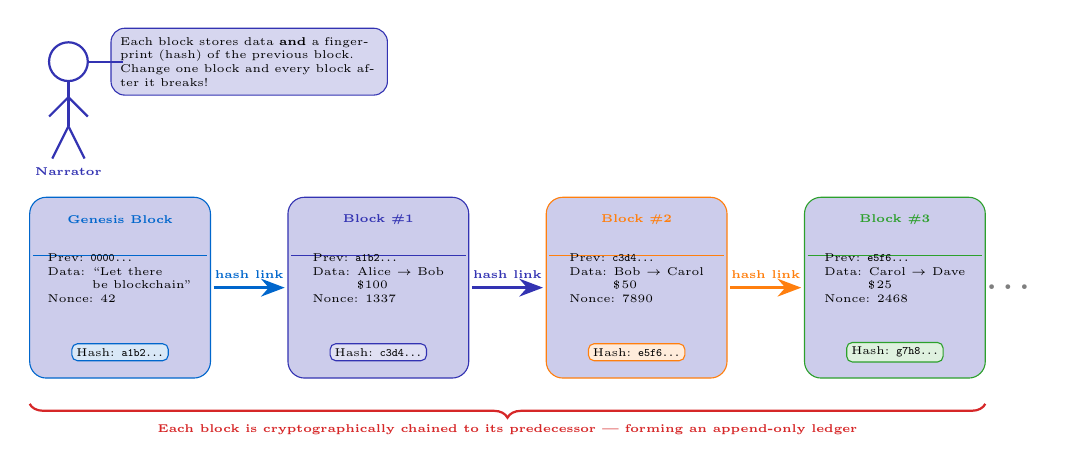
\begin{tikzpicture}[scale=0.82, every node/.style={transform shape}]

% --- Narrator character (top-left) ---
\draw[mlpurple, thick] (-6.8,3.0) circle (0.3);
\draw[mlpurple, thick] (-6.8,2.7) -- (-6.8,2.0);
\draw[mlpurple, thick] (-6.8,2.45) -- (-7.1,2.15);
\draw[mlpurple, thick] (-6.8,2.45) -- (-6.5,2.15);
\draw[mlpurple, thick] (-6.8,2.0) -- (-7.05,1.5);
\draw[mlpurple, thick] (-6.8,2.0) -- (-6.55,1.5);
\node[font=\tiny\bfseries, mlpurple] at (-6.8,1.3) {Narrator};

% Narrator speech bubble
\node[draw=mlpurple, fill=mllavender4, rounded corners=5pt, font=\tiny,
      text width=4.0cm, align=left, inner sep=4pt]
      at (-4.0,3.0) {Each block stores data \textbf{and} a fingerprint (hash) of the previous block. Change one block and every block after it breaks!};
\draw[mlpurple, thick] (-6.5,3.0) -- (-5.95,3.0);

% --- Genesis Block ---
\node[draw=mlblue, fill=mllavender3, rounded corners=6pt, minimum width=2.8cm,
      minimum height=2.8cm, inner sep=3pt] (block0) at (-6.0,-0.5) {};
\node[font=\tiny\bfseries, mlblue] at (-6.0,0.55) {Genesis Block};
\draw[mlblue, thin] (-7.35,-0.0) -- (-4.65,-0.0);
\node[font=\tiny, align=left] at (-6.0,-0.35) {%
  Prev: \texttt{0000...}\\
  Data: ``Let there\\
  \phantom{Data: }be blockchain''\\
  Nonce: 42};
\node[draw=mlblue, fill=mlblue!15, rounded corners=2pt, font=\tiny, inner sep=2pt]
      at (-6.0,-1.5) {Hash: \texttt{a1b2...}};

% --- Block 1 ---
\node[draw=mlpurple, fill=mllavender3, rounded corners=6pt, minimum width=2.8cm,
      minimum height=2.8cm, inner sep=3pt] (block1) at (-2.0,-0.5) {};
\node[font=\tiny\bfseries, mlpurple] at (-2.0,0.55) {Block \#1};
\draw[mlpurple, thin] (-3.35,-0.0) -- (-0.65,-0.0);
\node[font=\tiny, align=left] at (-2.0,-0.35) {%
  Prev: \texttt{a1b2...}\\
  Data: Alice $\to$ Bob\\
  \phantom{Data: }\$100\\
  Nonce: 1337};
\node[draw=mlpurple, fill=mlpurple!15, rounded corners=2pt, font=\tiny, inner sep=2pt]
      at (-2.0,-1.5) {Hash: \texttt{c3d4...}};

% Hash arrow 0 -> 1
\draw[-{Stealth[length=3mm]}, mlblue, very thick]
      (-4.55,-0.5) -- (-3.45,-0.5)
      node[midway, above, font=\tiny\bfseries, mlblue] {hash link};

% --- Block 2 ---
\node[draw=mlorange, fill=mllavender3, rounded corners=6pt, minimum width=2.8cm,
      minimum height=2.8cm, inner sep=3pt] (block2) at (2.0,-0.5) {};
\node[font=\tiny\bfseries, mlorange] at (2.0,0.55) {Block \#2};
\draw[mlorange, thin] (0.65,-0.0) -- (3.35,-0.0);
\node[font=\tiny, align=left] at (2.0,-0.35) {%
  Prev: \texttt{c3d4...}\\
  Data: Bob $\to$ Carol\\
  \phantom{Data: }\$50\\
  Nonce: 7890};
\node[draw=mlorange, fill=mlorange!15, rounded corners=2pt, font=\tiny, inner sep=2pt]
      at (2.0,-1.5) {Hash: \texttt{e5f6...}};

% Hash arrow 1 -> 2
\draw[-{Stealth[length=3mm]}, mlpurple, very thick]
      (-0.55,-0.5) -- (0.55,-0.5)
      node[midway, above, font=\tiny\bfseries, mlpurple] {hash link};

% --- Block 3 ---
\node[draw=mlgreen, fill=mllavender3, rounded corners=6pt, minimum width=2.8cm,
      minimum height=2.8cm, inner sep=3pt] (block3) at (6.0,-0.5) {};
\node[font=\tiny\bfseries, mlgreen] at (6.0,0.55) {Block \#3};
\draw[mlgreen, thin] (4.65,-0.0) -- (7.35,-0.0);
\node[font=\tiny, align=left] at (6.0,-0.35) {%
  Prev: \texttt{e5f6...}\\
  Data: Carol $\to$ Dave\\
  \phantom{Data: }\$25\\
  Nonce: 2468};
\node[draw=mlgreen, fill=mlgreen!15, rounded corners=2pt, font=\tiny, inner sep=2pt]
      at (6.0,-1.5) {Hash: \texttt{g7h8...}};

% Hash arrow 2 -> 3
\draw[-{Stealth[length=3mm]}, mlorange, very thick]
      (3.45,-0.5) -- (4.55,-0.5)
      node[midway, above, font=\tiny\bfseries, mlorange] {hash link};

% Dots for continuation
\node[font=\Large\bfseries, mlgray] at (7.8,-0.5) {\ldots};

% --- Bottom annotation: chain property ---
\draw[mlred, thick, decorate, decoration={brace, amplitude=5pt, mirror}]
     (-7.4,-2.3) -- (7.4,-2.3);
\node[font=\tiny\bfseries, mlred] at (0.0,-2.7)
     {Each block is cryptographically chained to its predecessor --- forming an append-only ledger};

\end{tikzpicture}
\end{center}

\bottomnote{Source: Nakamoto, S. (2008). ``Bitcoin: A Peer-to-Peer Electronic Cash System.'' Each block's hash includes the previous block's hash, creating an unbreakable chain.}
\end{frame}

% ==================== FRAME 4: IMMUTABILITY ====================
\begin{frame}{Immutability: Why You Cannot Cheat}
\vspace{-2mm}
\begin{center}
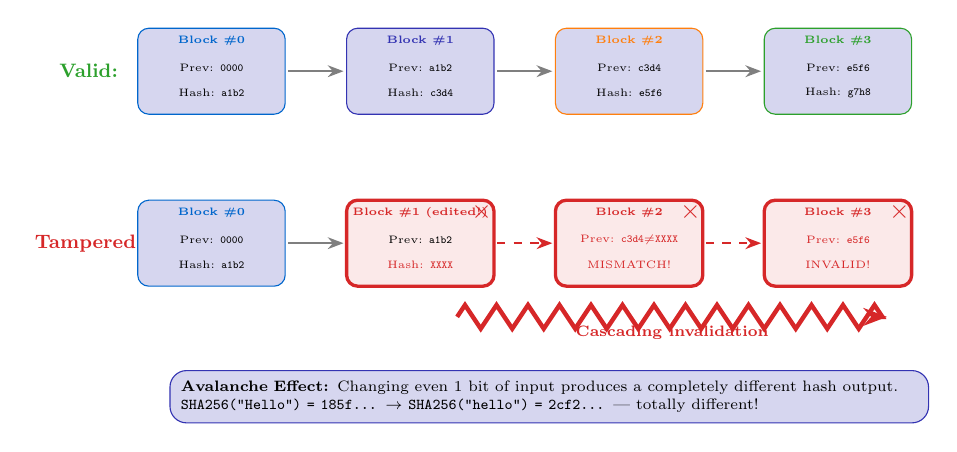
\begin{tikzpicture}[scale=0.78, every node/.style={transform shape}]

% === Row 1: Valid chain ===
\node[font=\small\bfseries, mlgreen] at (-7.5,2.5) {Valid:};

\foreach \i/\col/\hash/\prev in {0/mlblue/a1b2/0000, 1/mlpurple/c3d4/a1b2, 2/mlorange/e5f6/c3d4, 3/mlgreen/g7h8/e5f6} {
    \pgfmathsetmacro{\xpos}{-5.5 + \i * 3.4}
    \node[draw=\col, fill=mllavender4, rounded corners=4pt,
          minimum width=2.4cm, minimum height=1.4cm, inner sep=2pt]
          (v\i) at (\xpos,2.5) {};
    \node[font=\tiny\bfseries, \col] at (\xpos,3.0) {Block \#\i};
    \node[font=\tiny] at (\xpos,2.55) {Prev: \texttt{\prev}};
    \node[font=\tiny] at (\xpos,2.15) {Hash: \texttt{\hash}};
    % Checkmark
    \node[font=\small, mlgreen] at (\xpos + 1.0,3.0) {\checkmark};
}
% Arrows
\foreach \i in {0,1,2} {
    \pgfmathsetmacro{\xfrom}{-5.5 + \i * 3.4 + 1.25}
    \pgfmathsetmacro{\xto}{-5.5 + (\i+1) * 3.4 - 1.25}
    \draw[-{Stealth[length=2mm]}, mlgray, thick] (\xfrom,2.5) -- (\xto,2.5);
}

% === Row 2: Tampered chain ===
\node[font=\small\bfseries, mlred] at (-7.5,-0.3) {Tampered:};

% Block 0 unchanged
\node[draw=mlblue, fill=mllavender4, rounded corners=4pt,
      minimum width=2.4cm, minimum height=1.4cm, inner sep=2pt]
      (t0) at (-5.5,-0.3) {};
\node[font=\tiny\bfseries, mlblue] at (-5.5,0.2) {Block \#0};
\node[font=\tiny] at (-5.5,-0.25) {Prev: \texttt{0000}};
\node[font=\tiny] at (-5.5,-0.65) {Hash: \texttt{a1b2}};
\node[font=\small, mlgreen] at (-4.5,0.2) {\checkmark};

% Block 1 TAMPERED
\node[draw=mlred, fill=mlred!10, rounded corners=4pt, very thick,
      minimum width=2.4cm, minimum height=1.4cm, inner sep=2pt]
      (t1) at (-2.1,-0.3) {};
\node[font=\tiny\bfseries, mlred] at (-2.1,0.2) {Block \#1 (edited!)};
\node[font=\tiny] at (-2.1,-0.25) {Prev: \texttt{a1b2}};
\node[font=\tiny, mlred] at (-2.1,-0.65) {Hash: \texttt{XXXX}};
\node[font=\large\bfseries, mlred] at (-1.1,0.2) {$\times$};

% Block 2 broken
\node[draw=mlred, fill=mlred!10, rounded corners=4pt, very thick,
      minimum width=2.4cm, minimum height=1.4cm, inner sep=2pt]
      (t2) at (1.3,-0.3) {};
\node[font=\tiny\bfseries, mlred] at (1.3,0.2) {Block \#2};
\node[font=\tiny, mlred] at (1.3,-0.25) {Prev: \texttt{c3d4}$\neq$\texttt{XXXX}};
\node[font=\tiny, mlred] at (1.3,-0.65) {MISMATCH!};
\node[font=\large\bfseries, mlred] at (2.3,0.2) {$\times$};

% Block 3 broken
\node[draw=mlred, fill=mlred!10, rounded corners=4pt, very thick,
      minimum width=2.4cm, minimum height=1.4cm, inner sep=2pt]
      (t3) at (4.7,-0.3) {};
\node[font=\tiny\bfseries, mlred] at (4.7,0.2) {Block \#3};
\node[font=\tiny, mlred] at (4.7,-0.25) {Prev: \texttt{e5f6}};
\node[font=\tiny, mlred] at (4.7,-0.65) {INVALID!};
\node[font=\large\bfseries, mlred] at (5.7,0.2) {$\times$};

% Arrows with break
\draw[-{Stealth[length=2mm]}, mlgray, thick] (-4.25,-0.3) -- (-3.35,-0.3);
\draw[-{Stealth[length=2mm]}, mlred, thick, dashed] (-0.85,-0.3) -- (0.05,-0.3);
\draw[-{Stealth[length=2mm]}, mlred, thick, dashed] (2.55,-0.3) -- (3.45,-0.3);

% Cascading invalidation arrow
\draw[-{Stealth[length=3mm]}, mlred, ultra thick, decorate,
      decoration={zigzag, segment length=4mm, amplitude=1.5mm}]
      (-1.5,-1.5) -- (5.5,-1.5)
      node[midway, below, font=\scriptsize\bfseries, mlred] {Cascading invalidation};

% === Avalanche effect box ===
\node[draw=mlpurple, fill=mllavender4, rounded corners=6pt, inner sep=5pt,
      text width=12cm, align=left, font=\scriptsize]
      at (0.0,-2.8) {%
\textbf{Avalanche Effect:} Changing even 1 bit of input produces a completely different hash output.
\texttt{SHA256("Hello") = 185f...} $\to$ \texttt{SHA256("hello") = 2cf2...} --- totally different!};

\end{tikzpicture}
\end{center}

\bottomnote{Key insight: Tampering with one block invalidates every subsequent block, making fraud computationally infeasible.}
\end{frame}

% ==================== FRAME 5: CONSENSUS ====================
\begin{frame}{Consensus: How the Network Agrees}
\vspace{-2mm}
\begin{center}
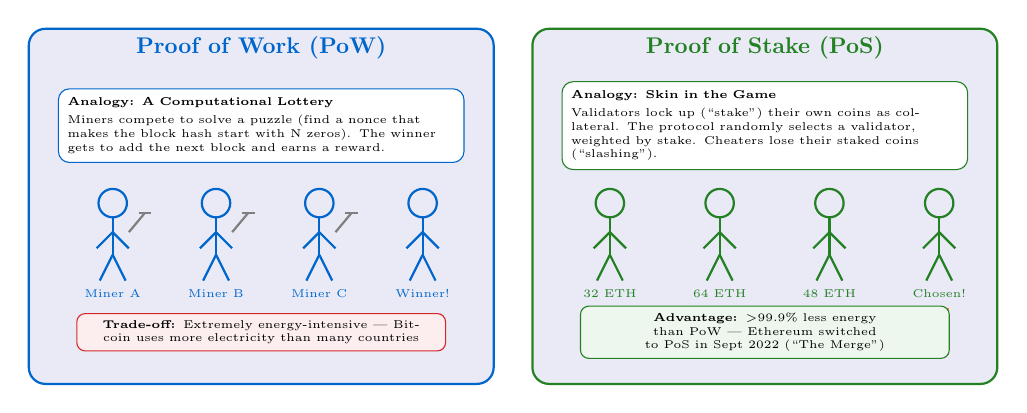
\begin{tikzpicture}[scale=0.82, every node/.style={transform shape}]

% Left half: Proof of Work
\draw[mlblue, thick, rounded corners=6pt, fill=mllavender4!50] (-7.5,-2.5) rectangle (-0.3,3.0);
\node[font=\normalsize\bfseries, mlblue] at (-3.9,2.7) {Proof of Work (PoW)};

% Lottery analogy
\node[draw=mlblue, fill=white, rounded corners=4pt, inner sep=4pt,
      text width=6.0cm, align=left, font=\tiny] at (-3.9,1.5) {%
\textbf{Analogy: A Computational Lottery}\\[2pt]
Miners compete to solve a puzzle (find a nonce that makes the block hash start with N zeros).
The winner gets to add the next block and earns a reward.};

% Miner stick figures
\foreach \i/\xoff/\label in {1/-6.2/Miner A, 2/-4.6/Miner B, 3/-3.0/Miner C, 4/-1.4/Winner!} {
    \pgfmathsetmacro{\ybase}{-0.5}
    \draw[mlblue, thick] (\xoff,\ybase+0.8) circle (0.22);
    \draw[mlblue, thick] (\xoff,\ybase+0.58) -- (\xoff,\ybase+0.0);
    \draw[mlblue, thick] (\xoff,\ybase+0.35) -- (\xoff-0.25,\ybase+0.1);
    \draw[mlblue, thick] (\xoff,\ybase+0.35) -- (\xoff+0.25,\ybase+0.1);
    \draw[mlblue, thick] (\xoff,\ybase+0.0) -- (\xoff-0.2,\ybase-0.4);
    \draw[mlblue, thick] (\xoff,\ybase+0.0) -- (\xoff+0.2,\ybase-0.4);
    \node[font=\tiny, mlblue] at (\xoff,\ybase-0.6) {\label};
}
% Pickaxe for miners
\foreach \xoff in {-6.2,-4.6,-3.0} {
    \draw[mlgray, thick] (\xoff+0.25,-0.15) -- (\xoff+0.5,0.15);
    \draw[mlgray, thick] (\xoff+0.4,0.15) -- (\xoff+0.6,0.15);
}
% Crown for winner
\node[font=\small, mlorange] at (-1.4,0.6) {$\bigstar$};

% Energy note
\node[draw=mlred, fill=mlred!8, rounded corners=3pt, font=\tiny,
      text width=5.5cm, align=center, inner sep=3pt] at (-3.9,-1.7) {%
\textbf{Trade-off:} Extremely energy-intensive --- Bitcoin uses more electricity than many countries};

% Right half: Proof of Stake
\draw[mlgreen!80!black, thick, rounded corners=6pt, fill=mllavender4!50] (0.3,-2.5) rectangle (7.5,3.0);
\node[font=\normalsize\bfseries, mlgreen!80!black] at (3.9,2.7) {Proof of Stake (PoS)};

% Staking analogy
\node[draw=mlgreen!80!black, fill=white, rounded corners=4pt, inner sep=4pt,
      text width=6.0cm, align=left, font=\tiny] at (3.9,1.5) {%
\textbf{Analogy: Skin in the Game}\\[2pt]
Validators lock up (``stake'') their own coins as collateral.
The protocol randomly selects a validator, weighted by stake.
Cheaters lose their staked coins (``slashing'').};

% Validator figures with coin stacks
\foreach \i/\xoff/\coins/\label in {1/1.5/2/32 ETH, 2/3.2/4/64 ETH, 3/4.9/3/48 ETH, 4/6.6/5/Chosen!} {
    \pgfmathsetmacro{\ybase}{-0.5}
    \draw[mlgreen!80!black, thick] (\xoff,\ybase+0.8) circle (0.22);
    \draw[mlgreen!80!black, thick] (\xoff,\ybase+0.58) -- (\xoff,\ybase+0.0);
    \draw[mlgreen!80!black, thick] (\xoff,\ybase+0.35) -- (\xoff-0.25,\ybase+0.1);
    \draw[mlgreen!80!black, thick] (\xoff,\ybase+0.35) -- (\xoff+0.25,\ybase+0.1);
    \draw[mlgreen!80!black, thick] (\xoff,\ybase+0.0) -- (\xoff-0.2,\ybase-0.4);
    \draw[mlgreen!80!black, thick] (\xoff,\ybase+0.0) -- (\xoff+0.2,\ybase-0.4);
    \node[font=\tiny, mlgreen!80!black] at (\xoff,\ybase-0.6) {\label};
    % Coin stack
    \foreach \c in {1,...,\coins} {
        \pgfmathsetmacro{\cy}{\ybase - 0.8 - \c*0.15}
        \draw[mlorange, fill=mlorange!30] (\xoff-0.15,\cy) rectangle (\xoff+0.15,\cy+0.12);
    }
}
% Arrow pointing to chosen
\node[font=\small, mlgreen!80!black] at (6.6,0.6) {$\bigstar$};

% Efficiency note
\node[draw=mlgreen!80!black, fill=mlgreen!8, rounded corners=3pt, font=\tiny,
      text width=5.5cm, align=center, inner sep=3pt] at (3.9,-1.7) {%
\textbf{Advantage:} $>$99.9\% less energy than PoW --- Ethereum switched to PoS in Sept 2022 (``The Merge'')};

\end{tikzpicture}
\end{center}

\bottomnote{Source: Ethereum Foundation, 2022. PoW secures via computational cost; PoS secures via economic penalty.}
\end{frame}

% ==================== FRAME 6: DECENTRALIZATION ====================
\begin{frame}{Decentralization: No Single Point of Failure}
\vspace{-1mm}
\begin{center}
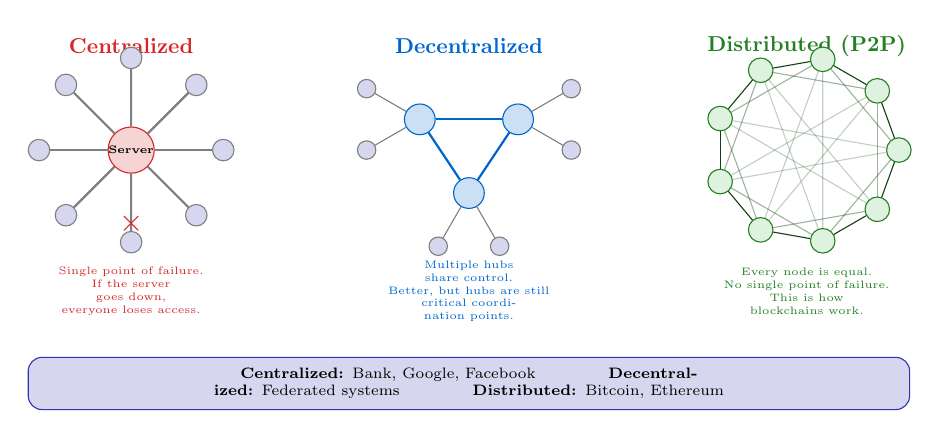
\begin{tikzpicture}[scale=0.78, every node/.style={transform shape}]

% === Centralized ===
\node[font=\normalsize\bfseries, mlred] at (-5.5,3.2) {Centralized};
% Central node
\node[draw=mlred, fill=mlred!20, circle, minimum size=0.7cm, inner sep=0pt,
      font=\tiny\bfseries] (c-center) at (-5.5,1.5) {Server};
% Peripheral nodes
\foreach \angle/\i in {0/1,45/2,90/3,135/4,180/5,225/6,270/7,315/8} {
    \node[draw=mlgray, fill=mllavender4, circle, minimum size=0.35cm, inner sep=0pt]
          (c-\i) at ($(-5.5,1.5)+(\angle:1.5)$) {};
    \draw[mlgray, thick] (c-center) -- (c-\i);
}
% X on center
\node[font=\Large\bfseries, mlred] at (-5.5,0.3) {$\times$};
\node[font=\tiny, mlred, text width=2.5cm, align=center] at (-5.5,-0.8) {%
Single point of failure.\\If the server goes down,\\everyone loses access.};

% === Decentralized ===
\node[font=\normalsize\bfseries, mlblue] at (0,3.2) {Decentralized};
% Multiple hubs
\foreach \pos/\name in {(-0.8,2.0)/H1,(0.8,2.0)/H2,(0,0.8)/H3} {
    \node[draw=mlblue, fill=mlblue!20, circle, minimum size=0.5cm, inner sep=0pt,
          font=\tiny] (\name) at \pos {};
}
% Connect hubs
\draw[mlblue, thick] (H1) -- (H2);
\draw[mlblue, thick] (H1) -- (H3);
\draw[mlblue, thick] (H2) -- (H3);
% Leaves
\foreach \hub/\angles in {H1/{150,210},H2/{-30,30},H3/{240,300}} {
    \foreach \a in \angles {
        \pgfmathsetmacro{\nodenum}{int(\a)}
        \node[draw=mlgray, fill=mllavender4, circle, minimum size=0.3cm, inner sep=0pt]
              (d-\hub-\nodenum) at ($(\hub)+(\a:1.0)$) {};
        \draw[mlgray] (\hub) -- (d-\hub-\nodenum);
    }
}
\node[font=\tiny, mlblue, text width=2.8cm, align=center] at (0,-0.8) {%
Multiple hubs share control.\\Better, but hubs are still\\critical coordination points.};

% === Distributed (Blockchain) ===
\node[font=\normalsize\bfseries, mlgreen!80!black] at (5.5,3.2) {Distributed (P2P)};
% Mesh network
\foreach \i/\angle in {1/0,2/40,3/80,4/120,5/160,6/200,7/240,8/280,9/320} {
    \node[draw=mlgreen!80!black, fill=mlgreen!15, circle, minimum size=0.4cm, inner sep=0pt]
          (p-\i) at ($(5.5,1.5)+(\angle:1.5)$) {};
}
% Mesh connections (every node connects to several others)
\foreach \i in {1,...,9} {
    \pgfmathsetmacro{\nexta}{int(mod(\i,9)+1)}
    \pgfmathsetmacro{\nextb}{int(mod(\i+1,9)+1)}
    \pgfmathsetmacro{\nextc}{int(mod(\i+3,9)+1)}
    \draw[mlgreen!40!black, thin] (p-\i) -- (p-\nexta);
    \draw[mlgreen!40!black, thin, opacity=0.4] (p-\i) -- (p-\nextb);
    \draw[mlgreen!40!black, thin, opacity=0.25] (p-\i) -- (p-\nextc);
}
% Highlight resilience
\node[font=\Large\bfseries, mlgreen!80!black] at (5.5,0.3) {\checkmark};
\node[font=\tiny, mlgreen!80!black, text width=2.8cm, align=center] at (5.5,-0.8) {%
Every node is equal.\\No single point of failure.\\This is how blockchains work.};

% Bottom comparison
\node[draw=mlpurple, fill=mllavender4, rounded corners=5pt, font=\scriptsize,
      text width=14cm, align=center, inner sep=5pt]
      at (0,-2.3) {%
\textbf{Centralized:} Bank, Google, Facebook \hspace{1cm}
\textbf{Decentralized:} Federated systems \hspace{1cm}
\textbf{Distributed:} Bitcoin, Ethereum};

\end{tikzpicture}
\end{center}

\bottomnote{Key insight: True decentralization means no entity can unilaterally censor, modify, or halt the network.}
\end{frame}

% ==================== FRAME 7: THE 51% ATTACK ====================
\begin{frame}{Risks: The 51\% Attack}
\vspace{-1mm}
\begin{columns}[T]
\column{0.48\textwidth}
\begin{center}
\textbf{\color{mlpurple}Hash Power Distribution}\\[4mm]
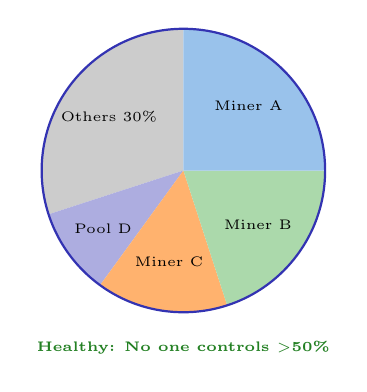
\begin{tikzpicture}[scale=0.9]
  % Pie chart for normal state
  % Slices: Miner A 25%, Miner B 20%, Miner C 15%, Pool D 10%, Others 30%
  \def\radius{2.0}

  % Others: 0-108 degrees (30%)
  \fill[mlgray!40] (0,0) -- (90:\radius) arc (90:198:\radius) -- cycle;
  \node[font=\tiny] at (144:1.3) {Others 30\%};

  % Pool D: 108-144 degrees (10%)
  \fill[mllavender] (0,0) -- (198:\radius) arc (198:234:\radius) -- cycle;
  \node[font=\tiny] at (216:1.4) {Pool D};

  % Miner C: 144-198 degrees (15%)
  \fill[mlorange!60] (0,0) -- (234:\radius) arc (234:288:\radius) -- cycle;
  \node[font=\tiny] at (261:1.3) {Miner C};

  % Miner B: 198-270 degrees (20%)
  \fill[mlgreen!40] (0,0) -- (288:\radius) arc (288:360:\radius) -- cycle;
  \node[font=\tiny] at (324:1.3) {Miner B};

  % Miner A: 270-360 degrees (25%)
  \fill[mlblue!40] (0,0) -- (0:\radius) arc (0:90:\radius) -- cycle;
  \node[font=\tiny] at (45:1.3) {Miner A};

  \draw[mlpurple, thick] (0,0) circle (\radius);
  \node[font=\tiny\bfseries, mlgreen!80!black] at (0,-2.5) {Healthy: No one controls $>$50\%};
\end{tikzpicture}
\end{center}

\column{0.48\textwidth}
\begin{center}
\textbf{\color{mlred}Attack Scenario}\\[3mm]
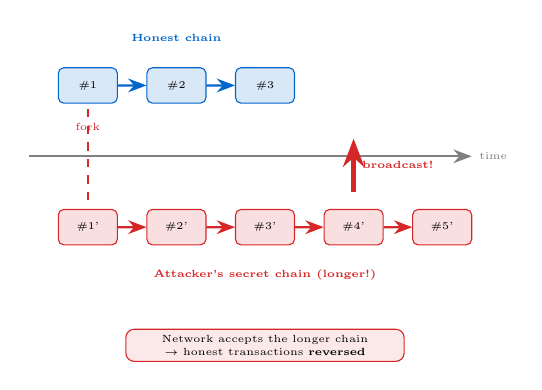
\begin{tikzpicture}[scale=0.75, every node/.style={transform shape}]
  % Timeline
  \draw[mlgray, thick, -{Stealth}] (-0.5,0) -- (7,0) node[right, font=\tiny] {time};

  % Honest chain
  \foreach \i/\x in {1/0.5, 2/2.0, 3/3.5} {
      \node[draw=mlblue, fill=mlblue!15, rounded corners=2pt,
            minimum width=1.0cm, minimum height=0.6cm, font=\tiny]
            (h\i) at (\x,1.2) {\#\i};
  }
  \draw[-{Stealth}, mlblue, thick] (h1) -- (h2);
  \draw[-{Stealth}, mlblue, thick] (h2) -- (h3);
  \node[font=\tiny\bfseries, mlblue] at (2.0,2.0) {Honest chain};

  % Attacker's secret chain (longer)
  \foreach \i/\x in {1/0.5, 2/2.0, 3/3.5, 4/5.0, 5/6.5} {
      \node[draw=mlred, fill=mlred!15, rounded corners=2pt,
            minimum width=1.0cm, minimum height=0.6cm, font=\tiny]
            (a\i) at (\x,-1.2) {\#\i'};
  }
  \draw[-{Stealth}, mlred, thick] (a1) -- (a2);
  \draw[-{Stealth}, mlred, thick] (a2) -- (a3);
  \draw[-{Stealth}, mlred, thick] (a3) -- (a4);
  \draw[-{Stealth}, mlred, thick] (a4) -- (a5);
  \node[font=\tiny\bfseries, mlred] at (3.5,-2.0) {Attacker's secret chain (longer!)};

  % Fork point
  \draw[mlred, thick, dashed] (0.5,0.8) -- (0.5,-0.8);
  \node[font=\tiny, mlred] at (0.5,0.5) {fork};

  % Broadcast arrow
  \draw[-{Stealth}, mlred, ultra thick] (5.0,-0.6) -- (5.0,0.3)
        node[midway, right, font=\tiny\bfseries, mlred] {broadcast!};

  % Result
  \node[draw=mlred, fill=mlred!10, rounded corners=3pt, font=\tiny,
        text width=4.5cm, align=center, inner sep=3pt] at (3.5,-3.2) {%
  Network accepts the longer chain\\$\to$ honest transactions \textbf{reversed}};
\end{tikzpicture}
\end{center}
\end{columns}

\vspace{2mm}
\begin{block}{\small Mitigation Strategies}
\begin{itemize}\scriptsize
    \item Wait for multiple confirmations (Bitcoin: 6 blocks $\approx$ 60 minutes)
    \item Economic cost: attacking Bitcoin would require \$billions in hardware
    \item PoS makes attacks even costlier (attacker's stake gets ``slashed'')
\end{itemize}
\end{block}

\bottomnote{Source: Majority attacks have occurred on smaller chains (Ethereum Classic, 2019; Bitcoin Gold, 2018).}
\end{frame}

% ==================== FRAME 8: SCALABILITY TRILEMMA ====================
\begin{frame}{The Scalability Trilemma}
\vspace{-1mm}
\begin{center}
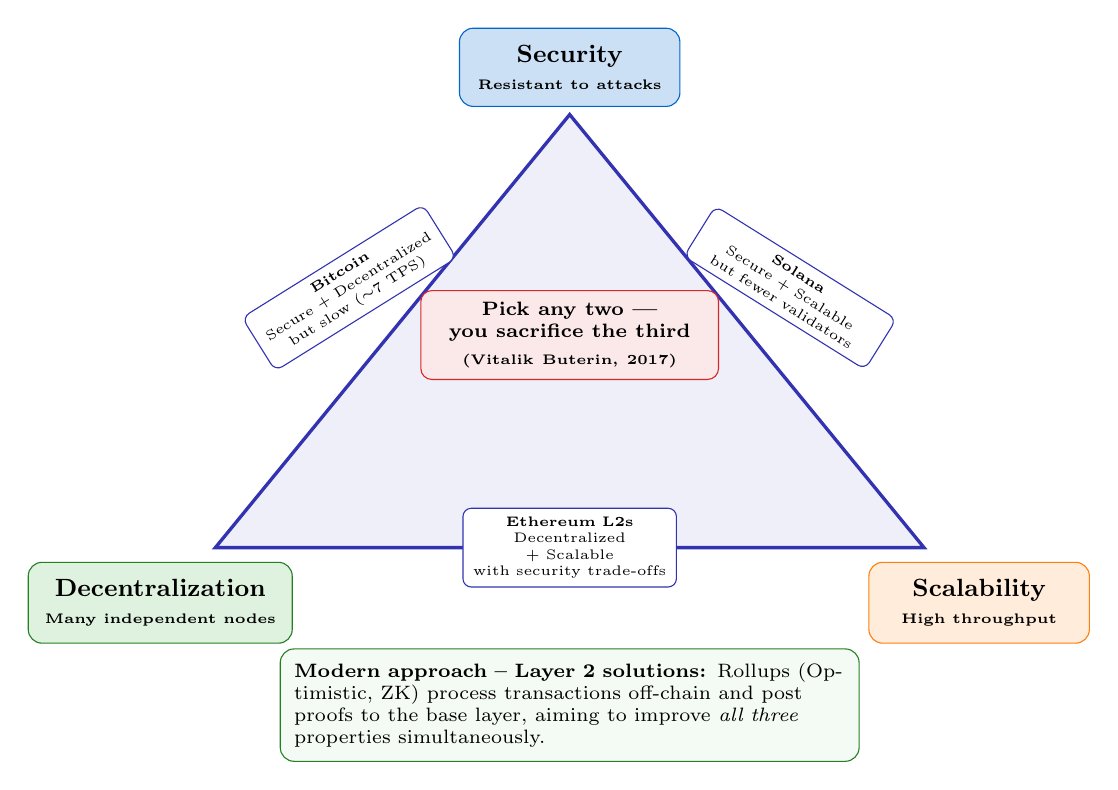
\begin{tikzpicture}[scale=1.0, every node/.style={transform shape}]

  % Main triangle
  \coordinate (top) at (0,4);
  \coordinate (bl) at (-4.5,-1.5);
  \coordinate (br) at (4.5,-1.5);

  % Filled triangle background
  \fill[mllavender4, opacity=0.4] (top) -- (bl) -- (br) -- cycle;
  \draw[mlpurple, very thick] (top) -- (bl) -- (br) -- cycle;

  % Vertex labels
  \node[draw=mlblue, fill=mlblue!20, rounded corners=5pt,
        font=\small\bfseries, inner sep=6pt, minimum width=2.8cm, align=center]
        (sec) at (0,4.6) {Security\\[-1pt]{\tiny Resistant to attacks}};

  \node[draw=mlgreen!80!black, fill=mlgreen!15, rounded corners=5pt,
        font=\small\bfseries, inner sep=6pt, minimum width=3.0cm, align=center]
        (dec) at (-5.2,-2.2) {Decentralization\\[-1pt]{\tiny Many independent nodes}};

  \node[draw=mlorange, fill=mlorange!15, rounded corners=5pt,
        font=\small\bfseries, inner sep=6pt, minimum width=2.8cm, align=center]
        (scl) at (5.2,-2.2) {Scalability\\[-1pt]{\tiny High throughput}};

  % Center label
  \node[draw=mlred, fill=mlred!10, rounded corners=4pt,
        font=\scriptsize\bfseries, inner sep=4pt, text width=3.5cm, align=center]
        at (0,1.2) {Pick any two ---\\you sacrifice the third\\[2pt]{\tiny (Vitalik Buterin, 2017)}};

  % Edge labels with blockchain examples
  \node[draw=mlpurple, fill=white, rounded corners=3pt,
        font=\tiny, inner sep=3pt, text width=2.5cm, align=center, rotate=32]
        at (-2.8,1.8) {\textbf{Bitcoin}\\Secure + Decentralized\\but slow ($\sim$7 TPS)};

  \node[draw=mlpurple, fill=white, rounded corners=3pt,
        font=\tiny, inner sep=3pt, text width=2.5cm, align=center, rotate=-32]
        at (2.8,1.8) {\textbf{Solana}\\Secure + Scalable\\but fewer validators};

  \node[draw=mlpurple, fill=white, rounded corners=3pt,
        font=\tiny, inner sep=3pt, text width=2.5cm, align=center]
        at (0,-1.5) {\textbf{Ethereum L2s}\\Decentralized + Scalable\\with security trade-offs};

  % Layer 2 note
  \node[draw=mlgreen!80!black, fill=mlgreen!5, rounded corners=5pt,
        font=\scriptsize, inner sep=5pt, text width=7cm, align=left]
        at (0,-3.5) {%
  \textbf{Modern approach -- Layer 2 solutions:} Rollups (Optimistic, ZK) process transactions off-chain and post proofs to the base layer, aiming to improve \emph{all three} properties simultaneously.};

\end{tikzpicture}
\end{center}

\bottomnote{Source: Buterin, V. (2017). The trilemma remains the central design challenge for all blockchain architectures.}
\end{frame}

% ==================== FRAME 9: BLOCKCHAIN BY THE NUMBERS (pgfplots) ====================
\begin{frame}{Blockchain by the Numbers: Transactions Per Second}
\vspace{-2mm}
\begin{center}
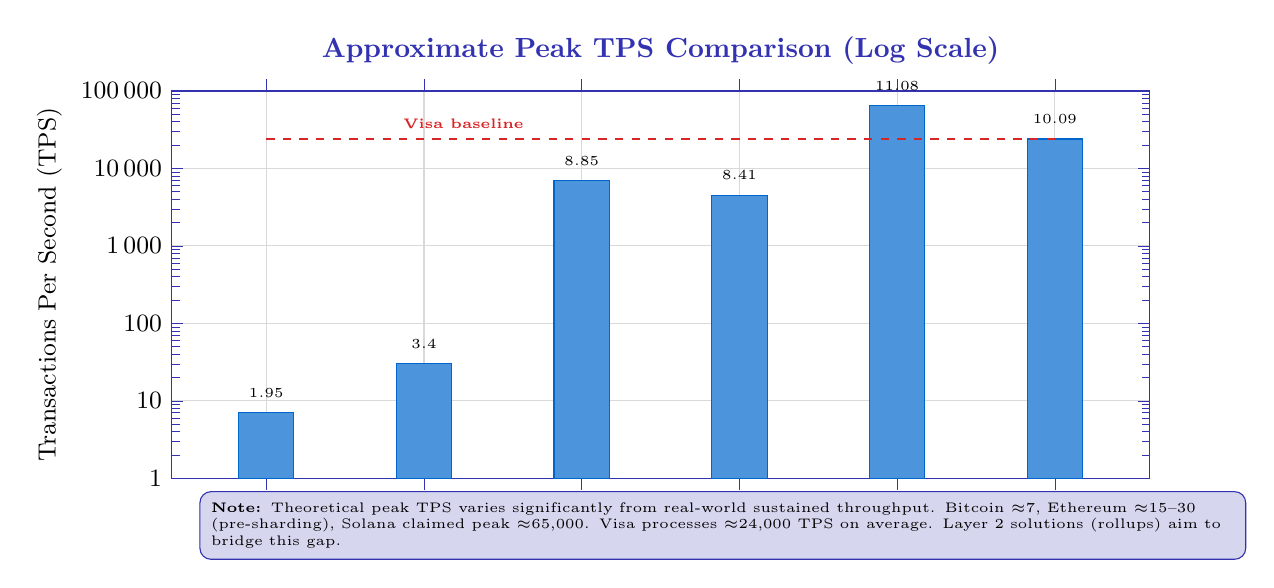
\begin{tikzpicture}
\begin{axis}[
    ybar,
    bar width=20pt,
    width=14cm,
    height=6.5cm,
    ymode=log,
    log origin=infty,
    ylabel={Transactions Per Second (TPS)},
    ylabel style={font=\small},
    xlabel style={font=\small},
    symbolic x coords={Bitcoin, Ethereum, Polygon, Avalanche, Solana, Visa},
    xtick=data,
    xticklabel style={font=\small, rotate=0},
    yticklabel style={font=\small},
    ymin=1,
    ymax=100000,
    ytick={1,10,100,1000,10000,100000},
    yticklabels={1,10,100,{1\,000},{10\,000},{100\,000}},
    nodes near coords,
    nodes near coords style={font=\tiny\bfseries, above, yshift=2pt},
    every node near coord/.append style={anchor=south},
    enlarge x limits=0.12,
    grid=major,
    major grid style={mlgray!30},
    axis line style={mlpurple},
    tick style={mlpurple},
    title style={font=\normalsize\bfseries, mlpurple},
    title={Approximate Peak TPS Comparison (Log Scale)},
    legend style={at={(0.02,0.98)}, anchor=north west, font=\tiny},
    clip=false,
]

% Blockchain bars
\addplot[fill=mlblue!70, draw=mlblue] coordinates {
    (Bitcoin,7) (Ethereum,30) (Polygon,7000) (Avalanche,4500)
    (Solana,65000) (Visa,24000)
};

% Annotation for reference
\draw[mlred, thick, dashed] (axis cs:Bitcoin,24000) -- (axis cs:Visa,24000)
      node[pos=0.25, above, font=\tiny\bfseries, mlred] {Visa baseline};

\end{axis}

% Note
\node[draw=mlpurple, fill=mllavender4, rounded corners=4pt, font=\tiny,
      text width=13cm, align=left, inner sep=4pt] at (7,-0.6) {%
\textbf{Note:} Theoretical peak TPS varies significantly from real-world sustained throughput.
Bitcoin $\approx$7, Ethereum $\approx$15--30 (pre-sharding), Solana claimed peak $\approx$65{,}000.
Visa processes $\approx$24{,}000 TPS on average. Layer 2 solutions (rollups) aim to bridge this gap.};

\end{tikzpicture}
\end{center}

\bottomnote{Source: Data approximate as of 2024. Actual throughput depends on network conditions, block size, and consensus parameters.}
\end{frame}

% ==================== FRAME 10: TAKEAWAYS AND EVALUATION FRAMEWORK ====================
\begin{frame}{Takeaways and Evaluation Framework}

\begin{columns}[T]
\column{0.48\textwidth}
\begin{block}{\small Key Concepts Covered}
\begin{enumerate}\small
    \item \textbf{Trust Problem} --- Why intermediaries are costly
    \item \textbf{Block Chaining} --- Hash-linked append-only ledger
    \item \textbf{Immutability} --- Tamper-evident via cryptographic hashing
    \item \textbf{Consensus} --- PoW (lottery) vs.\ PoS (stake)
    \item \textbf{Decentralization} --- No single point of failure
    \item \textbf{51\% Attack} --- Majority control risk
    \item \textbf{Scalability Trilemma} --- Security vs.\ decentralization vs.\ throughput
\end{enumerate}
\end{block}

\column{0.48\textwidth}
\begin{block}{\small 5-Point Evaluation Framework}
\textbf{For any blockchain project, ask:}\\[3mm]
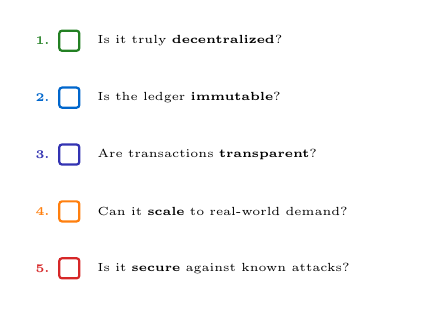
\begin{tikzpicture}[scale=0.85, every node/.style={transform shape}]
  \foreach \i/\q/\col in {
    1/{Is it truly \textbf{decentralized}?}/mlgreen!80!black,
    2/{Is the ledger \textbf{immutable}?}/mlblue,
    3/{Are transactions \textbf{transparent}?}/mlpurple,
    4/{Can it \textbf{scale} to real-world demand?}/mlorange,
    5/{Is it \textbf{secure} against known attacks?}/mlred} {
    \pgfmathsetmacro{\ypos}{3.0 - \i * 0.85}
    % Checkbox
    \draw[\col, thick, rounded corners=1pt] (-0.15,\ypos-0.15) rectangle (0.15,\ypos+0.15);
    % Question
    \node[font=\tiny, anchor=west, text width=4.5cm] at (0.3,\ypos) {\q};
    % Number
    \node[font=\tiny\bfseries, \col] at (-0.4,\ypos) {\i.};
  }
\end{tikzpicture}
\end{block}
\end{columns}

\vspace{3mm}
\begin{center}
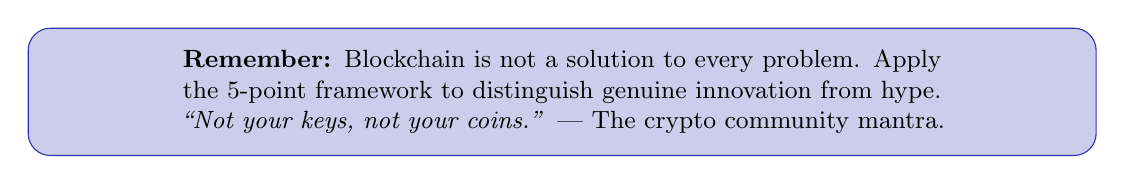
\begin{tikzpicture}
\node[draw=mlpurple, fill=mllavender3, rounded corners=8pt,
      font=\small, inner sep=8pt, text width=13cm, align=center] {%
\textbf{Remember:} Blockchain is not a solution to every problem.
Apply the 5-point framework to distinguish genuine innovation from hype.
\textit{``Not your keys, not your coins.''} --- The crypto community mantra.};
\end{tikzpicture}
\end{center}

\bottomnote{Key insight: A strong blockchain project should score well on all five criteria. Trade-offs are inevitable --- understand them.}
\end{frame}

\end{document}
